\section{Rendering und Physik}
	Das erste Problem ist das Darstellen des Spiels und die Interaktion zwischen den im Spiel existierenden Kugeln und dem Spielfeld. Zunächst schauen wir uns die Darstellung an.
\subsection{Objekte}
	Die Szene lässt sich einteilen in Löcher und Kugeln. Beide Strukturen werden aufgrund der Beschränkung auf 2D durch Kreise oder Kreisteile dargestellt. Dazu wird ein Triangle-Fan verwendet, der nun kurz erklärt werden soll.
	
	Ein Triangle-Fan zur Darstellung von Kreisen wird durch das Tripel Mittelpunkt $\mathbf{c}$, Radius $r$ und Anzahl der Unterteilungen $k$ parametrisiert. 
	Die Struktur beginnt im Punkt $(0,0)$.
	Das ist im Späteren Spielfeld der Punkt $\mathbf{c}$.
	Man gibt nun den Punkt an, bei dem das erste Dreieck beginnt. Dieser ist bei uns immer vertikal um r nach oben verschoben vom Mittelpunkt. Dann benötigt man noch einen Punkt um das Dreieck zu vollenden. Dieser Punkt ist im Uhrzeigersinn um $\delta$ auf dem Umriss verschoben. 
	$\delta$ ist der Grad, um den in jedem Schritt der Punkt auf dem Umriss verschoben wird. 
	Dabei muss gelten $\delta \cdot k = 360$ für einen ganzen Kreis.

	\begin{equation}\label{eq:delta}
		\delta =\frac{2 \cdot \pi}{k} 
	\end{equation}
	Sei $r$ der  Radius von der Kugel und $i$ der aktuelle Schritt in der Schleife von $i=1$ bis k, dann sind die Koordinaten für die Punkte auf dem Kreis:
	\begin{equation}\label{eq:circleCoord}
		\begin{aligned}
			x = \cos (\delta \cdot i) \cdot k\\
			y = \sin (\delta \cdot i) \cdot k
		\end{aligned}
	\end{equation}
	Für jeden Punkt der hinzugefügt wird, wird ein neues Dreieck erstellt, mit dem letzten Punkt, dem Mittelpunkt und dem neuen Punkt als Parameter.
	Wenn  nun $k$ mal die Koordinaten berechnet wurden, haben wir einen fertigen Kreis, bestehend aus $k$ Dreiecken.
		\begin{figure}[h]
		\centering
		\caption{Vollständiger Triangle-Fan mit k=12}
		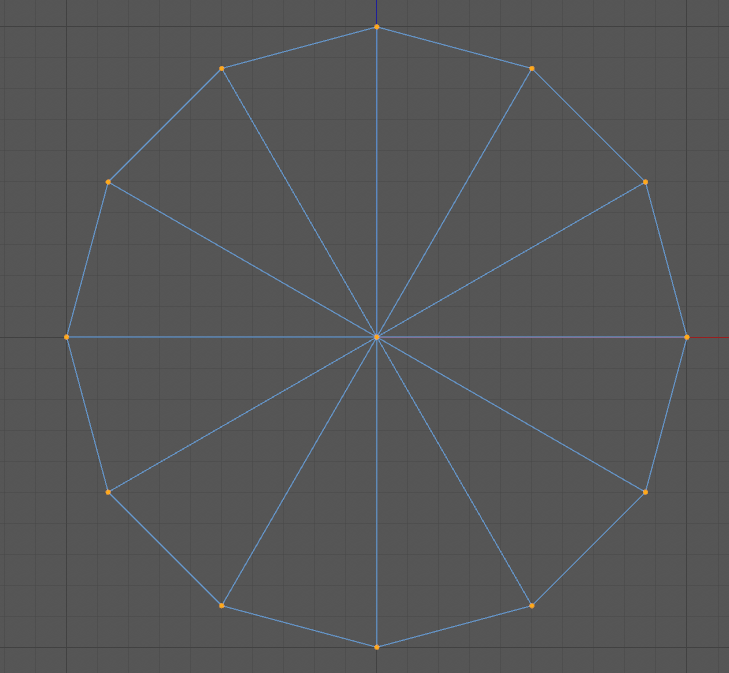
\includegraphics[width=\textwidth/6]{bilder/k12kreis.png} \\
	\end{figure} \\
	Die Triangle-Fans werden nun für die Löcher und Kugeln an den Positionen auf dem Spielfeld plaziert.
	\begin{figure}[h]
		\caption{Spielfeld ohne Texturen, mit k=64 für Triangle-Fans}
			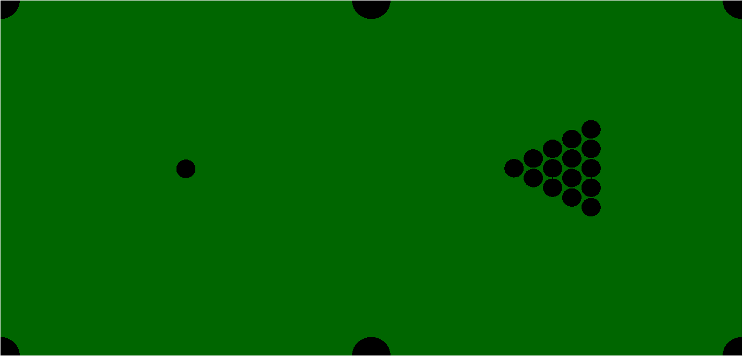
\includegraphics[width=\textwidth]{bilder/untextured_pool_low.png} 
	\end{figure}

\subsection{Texturierung}
	Die Farben für das Spielfeld sind trivial. 
	Die Kugeln hingegen müssen vom Spieler unterschieden werden können. 
	Wir müssen also Texturen auf Kreise abbilden. \\
	\begin{figure}[h]
		\caption{Billiardkugel Textur}
			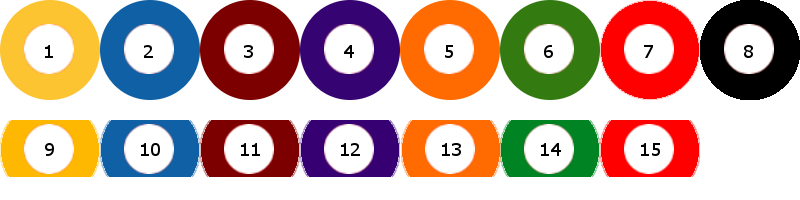
\includegraphics[width=\textwidth]{bilder/Balls.png} \\
	\end{figure} \\
	Um die Textur auf unsere Kugeln abzubilden verwenden wir u/v-Koordinaten. 
	Unsere Textur besitzt auf der $u$ und $v$ Achse einen Wertebereich von 0 bis 1. 
	Dabei ist $(0,0)$  oben links und $(1,1)$  unten rechts. 
	Jeder Kugel muss nun ein Ausschnitt der Textur zugewiesen werden. 
	Dafür bekommt jede Farbe einen Wert c.
	\begin{equation}\label{eq:color}
	c(b) = 
	\begin{cases}
		0, & \text{falls b Gelb} \\
		1, & \text{falls b Blau} \\
		2, & \text{falls b Rot} \\
		3, & \text{falls b Lila} \\
		4, & \text{falls b Orange} \\
		5, & \text{falls b Grün} \\
		6, & \text{falls b Rot} \\
		7, & \text{falls b Schwarz oder Weiß}
	\end{cases}
	\end{equation} 
	Außerdem bekommt jede Kugel einen Wert für die Fülle, wobei Voll = 0 ist und Halb = 1.  \\
	\begin{equation} \label{eq:full}
	f(b) = 
	\begin{cases}
		0, & \text{falls Kugel voll} \\
		1, & \text{falls Kugel halb}	
	\end{cases}
	\end{equation}\\
	\begin{figure}[h]
		\caption{Textur mit u/v-Koordinaten}
		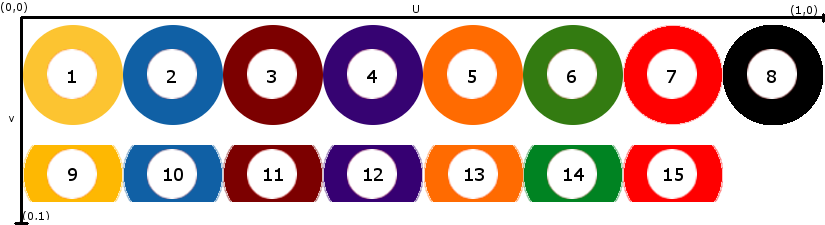
\includegraphics[width=\textwidth]{bilder/ballsachsen}
	\end{figure} \\
	Nun können wir uns eine Funktion erstellen, die anhand von Farbe und Fülle die Textur ausschneidet und auf die Kugel abbildet. 
	Dazu berechnen wir zuallererst die Anfangsposition der Textur. 
	Diese setzt sich zusammen aus der Farbe c und der Fülle f. \\
	Vorgedanke: Der Durchmesser einer Kugel auf unserer Textur ist $\frac{1}{8}$ für $u$, weil es 8 Kugeln pro Reihe gibt und die u Koordinate genau 1 lang ist. Der Durchmesser auf der $v$-Achse hingegen ist $\frac{1}{2}$, weil es nur 2 Reihen gibt und die Textur trotzdem 1 lang ist. \\
	Mittelpunkt m der Textur: \\
	\begin{equation}\label{eq:texStart}
	\begin{aligned} 
		x(b) = \frac{1}{16} + \frac{1}{8} \cdot c(b), c(b) = \text{Farbe der Kugel \eqref{eq:color}} \\
		y(b) = \frac{1}{4} + \frac{1}{2} \cdot f(b), f(b) = \text{Fülle der Kugel \eqref{eq:full}}
	\end{aligned}
	\end{equation}
	Nun fehlen noch die Texturkoordinaten für den Kreis um den Mittelpunkt der Textur herum.
	Die Berechnung läuft dabei analog zum Triangle-Fan mit dem Unterschied in der Skalierung und Startposition. 
	So benutzen wir nicht den Radius der Kugeln des Spiels, sondern die Größe der Kugel auf der Textur und als Startpunkt unser vorher berechnetes x und y in \eqref{eq:texStart}. 
	\begin{equation}\label{eq:texXY}
	\begin{aligned}
		 xTex(b) =  x(b) + \cos(\delta \cdot i) \cdot \frac{1}{16}, \\
		 yTex(b) =  y(b) + \sin(\delta \cdot i) \cdot \frac{1}{4}, \\
		\text{mit } \delta \text{ nach }\eqref{eq:delta} \text{ und } i \text{ nach } \eqref{eq:circleCoord}
	\end{aligned}
	\end{equation}
	Die Textur wird dann beim erstellen des Triangle-Fans auf die Dreiecke gezeichnet. Dabei bekommen die Dreiecke für den Mittelpunkt $(x,y)$ als Texturkoordinaten \eqref{eq:texStart} und der Punkt auf dem Umriss bekommt dann $(xTex,yTex)$ \eqref{eq:texXY}.
\subsection{Kollisionsberechnung}
	Die Kollisionsberechnung lässt sich aufteilen in 3 Bereiche: \begin{itemize}
		\item [1.] Kollision von Kugeln mit Wand und Löchern
		\item [2.] Kollision von Kugeln mit anderen Kugeln
		\item [3.] Kollision der Weißen Kugel mit dem Queue (Kapitel 3.3.3)
	\end{itemize}
	\subsubsection{Kollision von Kugeln mit Wand und Löchern}
		Das Kollidieren mit den Wänden ist sehr simpel: Wir geben  unsere Breite und Höhe des Spielfeldes als Grenzen an. Wenn die Kugel zu nah an eine der Wände kommt wird ihre Geschwindigkeit umgekehrt. Dementsprechend machen wir eine Fallunterscheidung mit 4 Fällen für die 4 verschiedenen Wände: \begin{itemize}
			\item [1.] Die Linke Wand (x=0)
			\item [2.] Die Rechte Wand (x=w)
			\item [3.] Die Obere Wand (y=0)
			\item [4.] Die untere Wand (y=h)
		\end{itemize}
		Dabei gilt $ h = $ Höhe des Spielfeldes, $ w = $ Breite des Spielfeldes und $l = $ Radius der Löcher.
		Die Änderung der Geschwindigkeit ist dann:
		\begin{equation}
		vy = \begin{cases}
			-vy, & \text{ falls } y \leq (h- l) \land y \geq l\\
			vy, & sonst 
		\end{cases}
		\end{equation}
		Das gilt für Fall 1 und 2. Für Fall 3 und 4 benötigen wir noch eine Bedingung mehr:
		 \begin{equation}
		vx = \begin{cases}
		-vx, & \text{ falls } (x \leq (w/2 - l) \land x \geq l) \lor (x \geq (w/2 + l) \land (x \leq (w- l) \\
		vx, & sonst 
		\end{cases}
		\end{equation}
		Wir überprüfen also, ob die Kugel eine der Beiden Strecken zwischen den Löchern trifft, wenn sie vorher den Rand des Spielfeldes erreicht hat. 
	\subsubsection{Kollision mit anderen Kugeln}
		Die Kollisionsberechnung für 2 Kugeln war uns bereits vorgegeben aus einem Beispiel für ein AirHockey Spiel. 
		Der Unterschied liegt darin, dass im Airhockey nur eine Kugel durch die Kollision ihre Geschwindigkeit ändert. Die beiden Schläger werden durch die Kollision nicht verändert. \\  
		Wir nehmen nun eine Kugel und berechnen mit der Methode alle Kollisionen mit anderen Kugeln, indem wir statt dem Schläger die jeweils andere Kugel einsetzen. Das muss für jede Kugel einmal ausgeführt werden.  \\
		
		%\begin{equation}
		%d = \sqrt{(x_2 - x_1)^2 + (y_2-y_1)^2} 
		%\end{equation}
		%Wenn diese Distanz kleiner ist als der Durchmesser $r*2$ einer Kugel, dann gibt es eine Kollision. \\
%		Die Kollision wird ausgewertet, indem zunächst die Normale berechnet wird: 
%		\begin{equation}
%		\begin{aligned}
%		nx = x_1 - x_2; \\
%		ny = y_1 - y_2; \\
%		\end{aligned}
%		\end{equation}
%		Das Ergebnis $(nx,ny)$  wird dann noch normalisiert. Dann berechnen wir die Tangente dazu:
%		\begin{equation}
%		\begin{aligned}
%		tx = -ny \\
%		ty = nx
%		\end{aligned}
%		\end{equation}
%		Als nächstes wird die Relative Geschwindigkeit zwischen beiden Kugeln berechnet. Dabei bezeichnen wir die Geschwindigkeit einer Kugel als vx bzw. vy (also $vx_1$ für die Geschwindigkeit auf der X-Achse der Kugel $b_1$).
%		\begin{equation}
%		\begin{aligned}
%		vrx = vx_2 - vx_1 \\
%		vry = vy_2 - vy_1
%		\end{aligned}
%		\end{equation}

	\subsubsection{Zusammenfassung}
		 Nun haben wir ein Spielfeld mit Texturierten Kugeln die miteinander kollidieren.
		 \begin{figure}[h]
		 	\caption{Fertiges Spielfeld}
		 	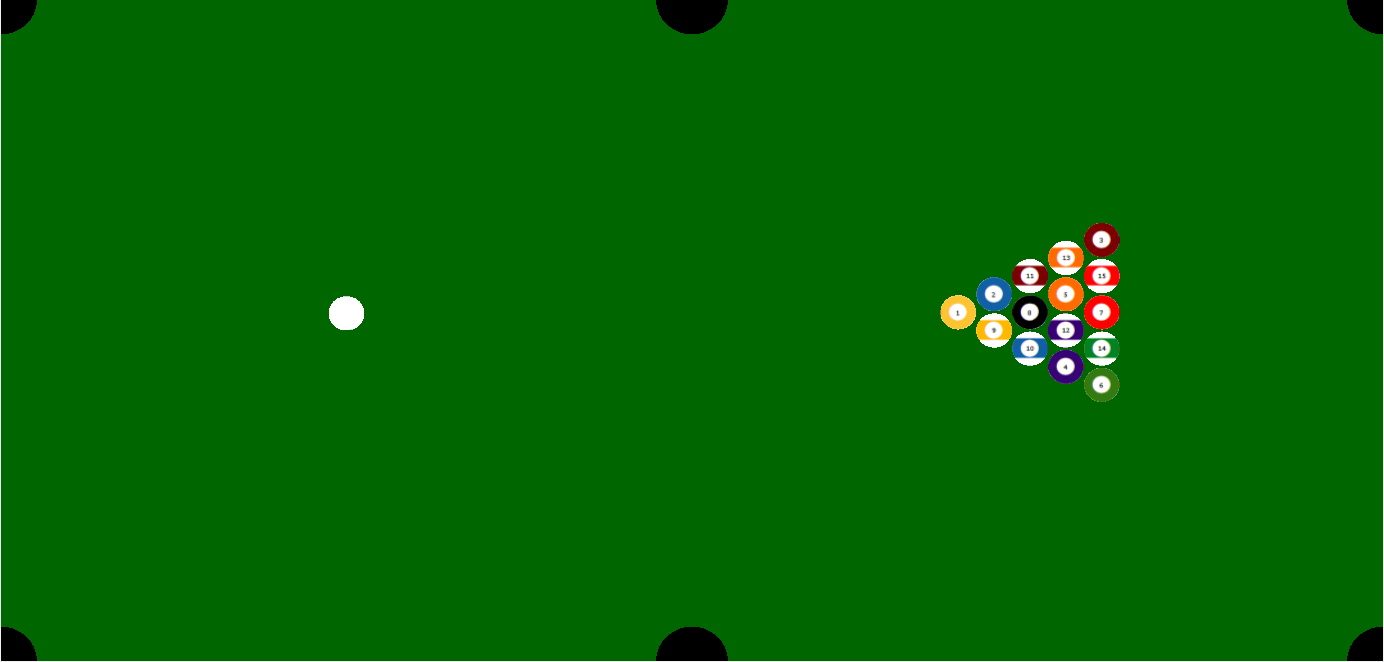
\includegraphics[width=\textwidth]{bilder/Spielfeld.png}
		 \end{figure}

